%!TEX options = --shell-escape


\documentclass[master]{thesis-uestc}

\title{时域积分方程时间步进算法及其快速算法}
\author{王稳}
\advisor{赖生建\chinesespace 副教授}
\school{物理电子学院}
\major{无线电物理}
\studentid{201421040223}

\begin{document}

\makecover

% this is a thesis template with mutiple files: the chapters and the misc in standalone mode
% to avoid too many files in current folder, template add extra direcotry: chapter and misc
% please do not change the sequence of each one except the chapters themselves.
% by FengYouzheng.

% abstract
\documentclass{standalone}
% preamble: usepackage, etc.
\begin{document}
	
\begin{chineseabstract}
为了适应日益增长的宽带信号和非线性系统的工程应用,用于分析瞬态电磁散射问题的时域积分方程方法研究日趋活跃。本文以时域积分方程时间步进算法及其快速算法为研究课题,重点研究了时间步进算法的数值实现技术、后时稳定性问题以及两层平面波算法加速计算等,主要研究内容分为四部分。

……

\chinesekeyword{时域电磁散射,时域积分方程,时间步进算法,后时不稳定性,时域平面波算法}
\end{chineseabstract}

\end{document}
\documentclass{standalone}
% preamble: usepackage, etc.
\begin{document}

\begin{englishabstract}
	With the widespread engineering applications ranging from broadband signals and non-linear systems, time-domain integral equations (TDIE) methods for analyzing transient electromagnetic scattering problems are becoming widely used nowadays. TDIE-based marching-on-in-time (MOT) scheme and its fast algorithm are researched in this dissertation, including the numerical techniques of MOT scheme, late-time stability of MOT scheme, and two-level PWTD-enhanced MOT scheme. The contents are divided into four parts shown as follows.
	
	\englishkeyword{time-domain electromagnetic scattering, time-domain integral equation (TDIE), marching-on in-time (MOT) scheme, late-time instability, plane wave time-domain (PWTD) algorithm}
\end{englishabstract}

\end{document}


% table of contents
\thesistableofcontents

% thesis contents
\documentclass{standalone}
% preamble: usepackage, etc.
\begin{document}

\thesischapterexordium

\section{研究工作的背景与意义}

计算电磁学方法\citing{wang1999sanwei, liuxf2006, zhu1973wulixue, chen2001hao, gu2012lao, feng997he}从时、频域角度划分可以分为频域方法与时域方法两大类。频域方法的研究开展较早,目前应用广泛的包括:矩量法(MOM)\citing{xiao2012yi,zhong1994zhong}及其快速算法多层快速多极子(MLFMA)\citing{clerc2010discrete}方法、有限元(FEM)\citing{wang1999sanwei,zhu1973wulixue}方法、自适应积分(AIM)\citing{gu2012lao}方法等,这些方法是目前计算电磁学商用软件
\footnote{脚注序号“\ding{172},……,\ding{180}”的字体是“正文”,不是“上标”,序号与脚注内容文字之间空1个半角字符,脚注的段落格式为:单倍行距,段前空0磅,段后空0磅,悬挂缩进1.5字符;中文用宋体,字号为小五号,英文和数字用Times New Roman字体,字号为9磅;中英文混排时,所有标点符号(例如逗号“,”、括号“()”等)一律使用中文输入状态下的标点符号,但小数点采用英文状态下的样式“.”。}
(例如:FEKO、Ansys 等)的核心算法。由文献\cite{feng997he,clerc2010discrete,xiao2012yi}可知

\section{时域积分方程方法的国内外研究历史与现状}
时域积分方程方法的研究始于上世纪60 年代,C.L.Bennet 等学者针对导体目
标的瞬态电磁散射问题提出了求解时域积分方程的时间步进(marching-on in-time,
MOT)算法。

\section{本文的主要贡献与创新}
本论文以时域积分方程时间步进算法的数值实现技术、后时稳定性问题以及两层平面波加速算法为重点研究内容,主要创新点与贡献如下:

\section{本论文的结构安排}
本文的章节结构安排如下:

\end{document}
\documentclass{standalone}
% preamble: usepackage, etc.
\begin{document}

\chapter{时域积分方程基础}
时域积分方程(TDIE)方法作为分析瞬态电磁波动现象最主要的数值算法之一,常用于求解均匀散射体和表面散射体的瞬态电磁散射问题。

\section{时域积分方程的类型}

\section{空间基函数与时间基函数}
利用数值算法求解时域积分方程,首先需要选取适当的空间基函数与时间基
函数对待求感应电流进行离散。

\subsection{空间基函数}
RWG 基函数是定义在三角形单元上的最具代表性的基函数。它的具体定义如
下:
\begin{equation}
f_n(r)=
\begin{cases}
\frac{l_n}{2A_n^+}\rho_n^+=\frac{l_n}{2A_n^+}(r-r_+)&r\in T_n^+\\
\frac{l_n}{2A_n^-}\rho_n^-=\frac{l_n}{2A_n^-}(r_--r)&r\in T_n^-\\
0&\text{otherwise}
\end{cases}
\end{equation}

其中,$l_n$为三角形单元$T_n^+$和$T_n^-$公共边的长度,$A_n^+$和$A_n^-$分别为三角形单元$T_n^+$和$T_n^-$的面积(如图\ref{pica}所示)。

\begin{figure}[h]
	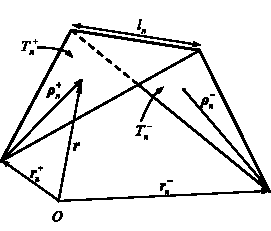
\includegraphics{pica.pdf}
	\caption{RWG 基函数几何参数示意图}
	\label{pica}
\end{figure}
由于时域混合场积分方程是时域电场积分方程与时域磁场积分方程的线性组合,因此时域混合场积分方程时间步进算法的阻抗矩阵特征与时域电场积分方程时间步进算法的阻抗矩阵特征相同。
\begin{equation}
\label{latent_binary_variable}
\mathbf{r}_{i,j}=
\begin{cases}
1,f(\mathbf{x}^{i};\mathbf{w})\cdot f(\mathbf{x}^{j};\mathbf{w})\geq u(\lambda),\\
0,f(\mathbf{x}^{i};\mathbf{w})\cdot f(\mathbf{x}^{j};\mathbf{w})< l(\lambda), 1\leq i,j\leq n.\\
f(\mathbf{x}^{i};\mathbf{w})\cdot f(\mathbf{x}^{j};\mathbf{w}),\text{otherwise},
\end{cases}
\end{equation}

时域积分方程时间步进算法的阻抗元素直接影响算法的后时稳定性,因此阻抗元素的计算是算法的关键之一,采用精度高效的方法计算时域阻抗元素是时域积分方程时间步进算法研究的重点之一。


\subsection{时间基函数}

\subsubsection{时域方法特有的展开函数}

\subsubsection{频域方法特有的展开函数}

\section{入射波}

如图\ref{picb}和图\ref{picc}所示分别给出了参数$E_0=\hat{x}$,$a_n=-\hat{z}$,$f_0=250MHz$,$f_w=50MHz$,$t_w=4.2\sigma$时,调制高斯脉冲的时域与频域归一化波形图。

\begin{figure}[h]
	\subfigure[]{
		\label{picb}
		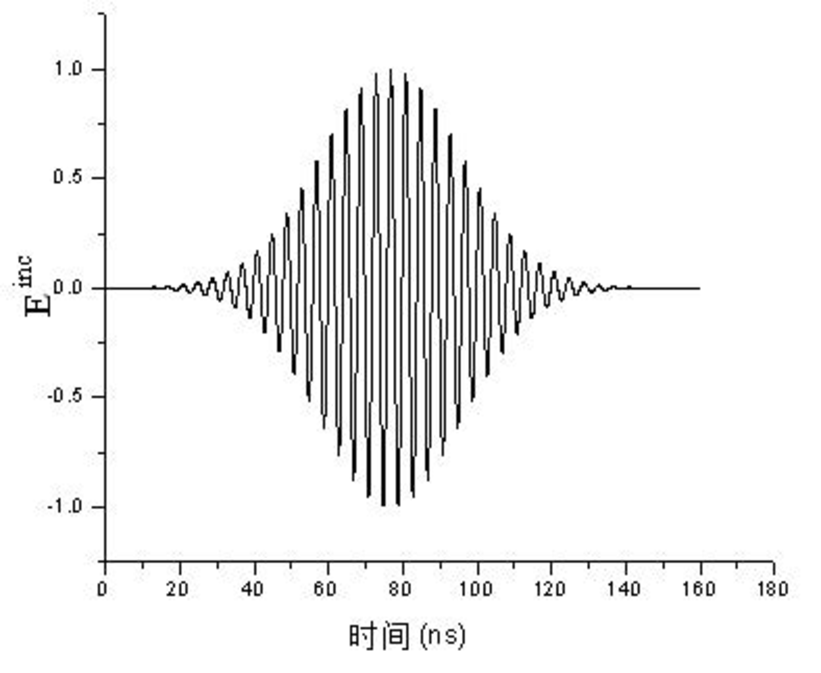
\includegraphics[width=7.3cm]{picb.pdf}}
	\subfigure[]{
		\label{picc}
		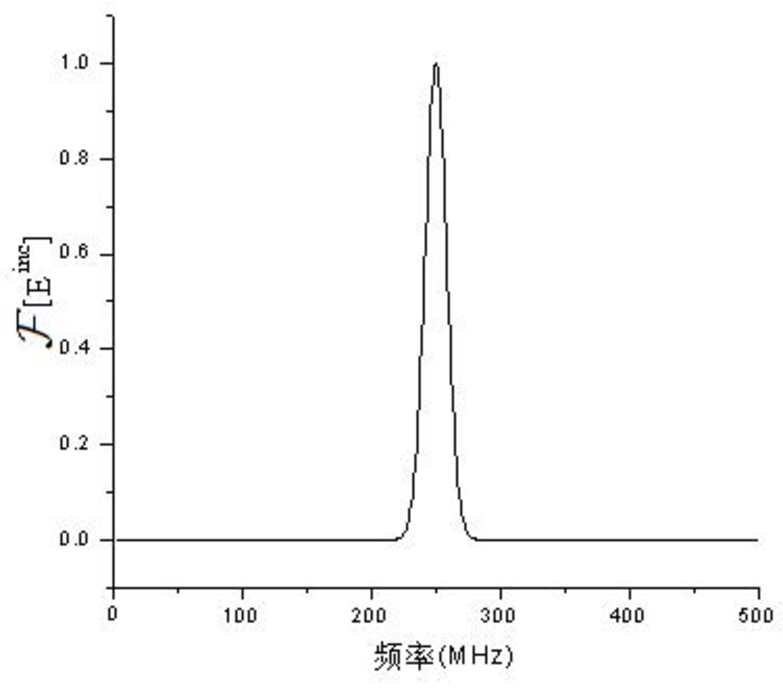
\includegraphics[width=6.41cm]{picc.pdf}}
	\caption{调制高斯脉冲时域与频率波形,时域阻抗元素的存储技术也是时间步进算法并行化的关键技术之一,采用合适的阻抗元素存储方式可以很大的提高并行时间步进算法的计算效率。}
	\label{fig1}
\end{figure}
时域阻抗元素的存储技术\citing{xiao2012yi}也是时间步进算法并行化的关键技术之一,采用合适的阻抗元素存储方式可以很大的提高并行时间步进算法的计算效率。

\section{本章小结}
本章首先从时域麦克斯韦方程组出发推导得到了时域电场、磁场以及混合场积分方程。

\chapter{时域积分方程数值方法研究}
\section{时域积分方程时间步进算法的阻抗元素精确计算}
时域积分方程时间步进算法的阻抗元素直接影响算法的后时稳定性,因此阻抗元素的计算是算法的关键之一,采用精度高效的方法计算时域阻抗元素是时域积分方程时间步进算法研究的重点之一。

\section{时域积分方程时间步进算法阻抗矩阵的存储}
时域阻抗元素的存储技术也是时间步进算法并行化的关键技术之一,采用合适的阻抗元素存储方式可以很大的提高并行时间步进算法的计算效率。

\subsection{时域积分方程时间步进算法产生的阻抗矩阵的特征}
由于时域混合场积分方程是时域电场积分方程与时域磁场积分方程的线性组合,因此时域混合场积分方程时间步进算法的阻抗矩阵特征与时域电场积分方程时间步进算法的阻抗矩阵特征相同。

\subsection{数值算例与分析}

如图3-1(a)所示给出了时间步长选取为0.5ns时采用三种不同存储方式计算的平板中心处 方向的感应电流值与IDFT方法计算结果的比较。如图3-1(b)所示给出了存储方式为基权函数压缩存储方式,时间步长分别取时平板中心处 方向的感应电流计算结果,从图中可以看出不同时间步长的计算结果基本相同。

\begin{algorithm}[H]
	\KwData{this text}
	\KwResult{how to write algorithm with \LaTeX2e }
	initialization\;
	\While{not at end of this document}{
		read current\;
		\eIf{understand}{
			go to next section\;
			current section becomes this one\;
		}{
		go back to the beginning of current section\;
	}
}
\caption{How to wirte an algorithm.}
\end{algorithm}

由于时域混合场积分方程是时域电场积分方程与时域磁场积分方程的线性组合,因此时域混合场积分方程时间步进算法的阻抗矩阵特征与时域电场积分方程时间步进算法的阻抗矩阵特征相同。

\section{时域积分方程时间步进算法矩阵方程的求解}

\section{本章小结}
本章首先研究了时域积分方程时间步进算法的阻抗元素精确计算技术,分别采用DUFFY变换法与卷积积分精度计算法计算时域阻抗元素,通过算例验证了计算方法的高精度。

\end{document}
\documentclass{standalone}
% preamble: usepackage, etc.
\begin{document}

\chapter{时域积分方程数值方法研究}
\section{时域积分方程时间步进算法的阻抗元素精确计算}
时域积分方程时间步进算法的阻抗元素直接影响算法的后时稳定性,因此阻抗元素的计算是算法的关键之一,采用精度高效的方法计算时域阻抗元素是时域积分方程时间步进算法研究的重点之一。

% \section{时域积分方程时间步进算法阻抗矩阵的存储}
% 时域阻抗元素的存储技术也是时间步进算法并行化的关键技术之一,采用合适的阻抗元素存储方式可以很大的提高并行时间步进算法的计算效率。

\subsection{时域积分方程时间步进算法产生的阻抗矩阵的特征}
由于时域混合场积分方程是时域电场积分方程与时域磁场积分方程的线性组合,因此时域混合场积分方程时间步进算法的阻抗矩阵特征与时域电场积分方程时间步进算法的阻抗矩阵特征相同。

\subsection{数值算例与分析}

如图3-1(a)所示给出了时间步长选取为0.5ns时采用三种不同存储方式计算的平板中心处 方向的感应电流值与IDFT方法计算结果的比较。如图3-1(b)所示给出了存储方式为基权函数压缩存储方式,时间步长分别取时平板中心处 方向的感应电流计算结果,从图中可以看出不同时间步长的计算结果基本相同。

\begin{algorithm}[H]
	\KwData{this text}
	\KwResult{how to write algorithm with \LaTeX2e }
	initialization\;
	\While{not at end of this document}{
		read current\;
		\eIf{understand}{
			go to next section\;
			current section becomes this one\;
		}{
		go back to the beginning of current section\;
	}
}
\caption{How to wirte an algorithm.}
\end{algorithm}

由于时域混合场积分方程是时域电场积分方程与时域磁场积分方程的线性组合,因此时域混合场积分方程时间步进算法的阻抗矩阵特征与时域电场积分方程时间步进算法的阻抗矩阵特征相同。

\section{时域积分方程时间步进算法矩阵方程的求解}

\section{本章小结}
本章首先研究了时域积分方程时间步进算法的阻抗元素精确计算技术,分别采用DUFFY变换法与卷积积分精度计算法计算时域阻抗元素,通过算例验证了计算方法的高精度。

\end{document}

\documentclass{standalone}
% preamble: usepackage, etc.
\begin{document}

\chapter{时域积分方程数值方法研究}
\section{时域积分方程时间步进算法的阻抗元素精确计算}
时域积分方程时间步进算法的阻抗元素直接影响算法的后时稳定性,因此阻
抗元素的计算是算法的关键之一,采用精度高效的方法计算时域阻抗元素是时域
积分方程时间步进算法研究的重点之一。

\section{时域积分方程时间步进算法阻抗矩阵的存储}
时域阻抗元素的存储技术也是时间步进算法并行化的关键技术之一,采用
合适的阻抗元素存储方式可以很大的提高并行时间步进算法的计算效率。

\subsection{时域积分方程时间步进算法产生的阻抗矩阵的特征}

由于时域混合场积分方程是时域电场积分方程与时域磁场积分方程的线性组
合,因此时域混合场积分方程时间步进算法的阻抗矩阵特征与时域电场积分方程
时间步进算法的阻抗矩阵特征相同。
\subsection{数值算例与分析}
如表\ref{tablea}所示给出了时间步长分别取0.4ns、0.5ns、0.6ns 时的三种存储
方式的存储量大小。

\begin{table}[h]
	\caption{计算$2m\times 2m$理想导体平板时域感应电流采用的三种存储方式的存储量比较。} 
	\begin{tabular}{|c|c|c|c|} 
		\hline  
		时间步长 & 非压缩存储方式 & 完全压缩存储方式 & 基权函数压缩存储方式 \\
		\hline 
		0.4ns & 5.59 MB & 6.78 MB & 6.78 MB\\  
		\hline  
		0.5ns & 10.17 MB & 5.58 MB & 5.58 MB \\  
		\hline  
		0.6ns & 8.38MB & 4.98 MB & 4.98 MB \\  
		\hline  
	\end{tabular}
	\label{tablea}
\end{table}

如图\ref{picd}所示给出了时间步长选取为0.5ns 时采用三种不同存储方式计算的
平板中心处$x$方向的感应电流值与IDFT 方法计算结果的比较,……。如图\ref{pice}
所示给出了存储方式为基权函数压缩存储方式,时间步长分别取0.4ns、0.5ns、0.6ns
时平板中心处$x$方向的感应电流计算结果,从图中可以看出不同时间步长的计算结果基本相同。

由于时域混合场积分方程是时域电场积分方程与时域磁场积分方程的线性组合,因此时域混合场积分方程时间步进算法的阻抗矩阵特征与时域电场积分方程时间步进算法的阻抗矩阵特征相同。

\begin{figure}[h]
	\subfigure[]{
		\label{picd}
		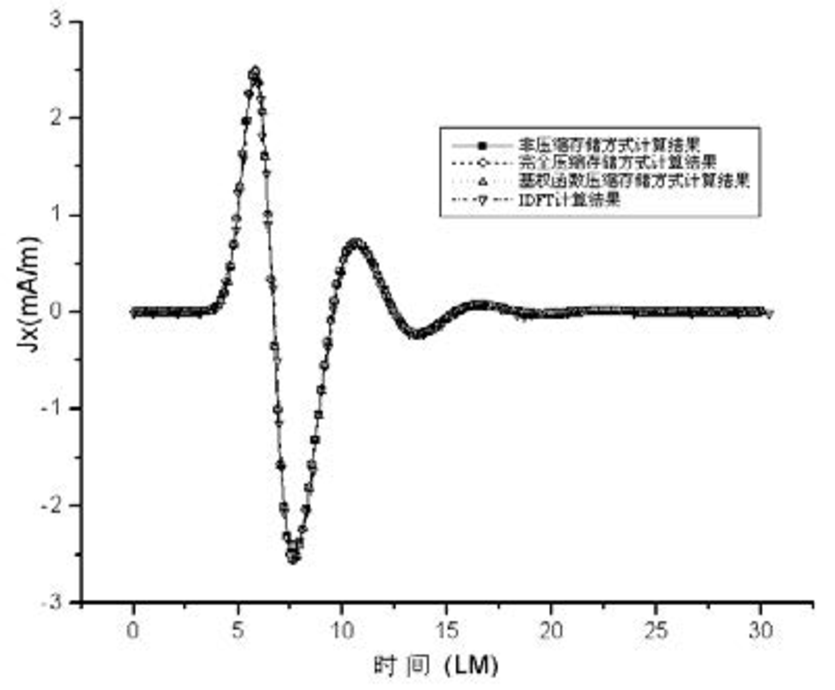
\includegraphics[width=6.77cm]{picd.pdf}}
	\subfigure[]{
		\label{pice}
		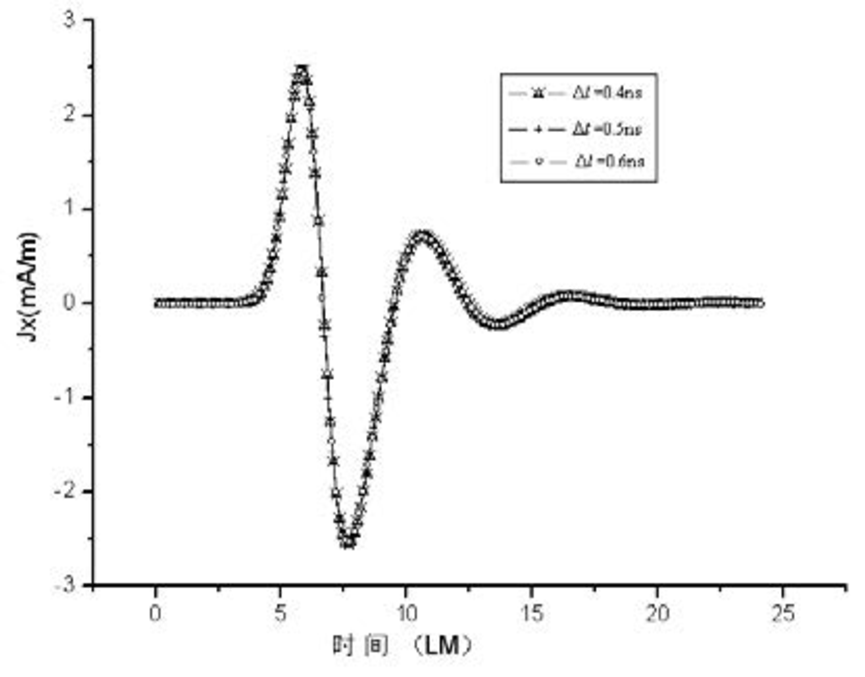
\includegraphics[width=7.04cm]{pice.pdf}}
	\caption{$2m\times 2m$的理想导体平板中心处感应电流$x$分量随时间的变化关系}
	\label{fig2}
\end{figure}


由于时域混合场积分方程是时域电场积分方程与时域磁场积分方程的线性组
合,因此时域混合场积分方程时间步进算法的阻抗矩阵特征与时域电场积分方程
时间步进算法的阻抗矩阵特征相同。
\section{时域积分方程时间步进算法矩阵方程的求解}

\begin{theorem}
	如果时域混合场积分方程是时域电场积分方程与时域磁场积分方程
	的线性组合。
\end{theorem}
\begin{proof}
	由于时域混合场积分方程是时域电场积分方程与时域磁场积分方程的线性组
	合,因此时域混合场积分方程时间步进算法的阻抗矩阵特征与时域电场积分方程
	时间步进算法的阻抗矩阵特征相同。
\end{proof}
\begin{corollary}
	时域积分方程方法的研究近几年发展迅速,在本文研究工作的基础上,仍有以下方向值得进一步研究。
\end{corollary}
\begin{lemma}
	因此时域混合场积分方程时间步进算法的阻抗矩阵特征与时域电场积分方程
	时间步进算法的阻抗矩阵特征相同。
\end{lemma}

\section{本章小结}
本章首先研究了时域积分方程时间步进算法的阻抗元素精确计算技术,分别
采用DUFFY 变换法与卷积积分精度计算法计算时域阻抗元素,通过算例验证了计
算方法的高精度。

\end{document}
\documentclass{standalone}
% preamble: usepackage, etc.
\begin{document}
	
\chapter{全文总结与展望}

\section{全文总结}
本文以时域积分方程方法为研究背景,主要对求解时域积分方程的时间步进算法以及两层平面波快速算法进行了研究。

\section{后续工作展望}
时域积分方程方法的研究近几年发展迅速,在本文研究工作的基础上,仍有以下方向值得进一步研究:

\end{document}
%\documentclass[12pt, UTF8, heading = false, scheme = plain]{ctexart}
    \usepackage{styles/zhtypo}

    \title{LaTeX 介绍}
    \author{维基百科}
    \date{\today}

    \begin{document}
    \pagestyle{empty} % 取消页码

    \clearpage\maketitle
    \thispagestyle{empty} % 去除首页页码

    文字形式写作LaTeX,是一种基于TEX的排版系统,由美国计算机科学家莱斯利·兰伯特在20世纪80年代初期开发,利用这种格式系统的处理,即使用户没有排版和程序设计的知识也可以充分发挥由TEX所提供的强大功能,不必一一亲自去设计或校对,能在几天,甚至几小时内生成很多具有书籍品质的印刷品。对于生成复杂表格和数学公式,这一点表现得尤为突出。因此它非常适用于生成高印刷质量的科技和数学、化学类文档。这个系统同样适用于生成从简单的信件到完整书籍的所有其他种类的文档。
    LATEX使用TEX作为它的格式化引擎。

    \section{排版系统}
    LaTeX遵循呈现与内容分离的设计理念,以便作者可以专注于他们正在编写的内容,而不必同时注视其外观。在准备LaTeX文档时,作者指定的逻辑结构使用简单的,熟悉的概念,如章(chapter),节(section),表(table),图(figure)等,并让LaTeX系统负责这些结构的格式和布局。因此,它鼓励从内容中分离布局,同时仍然允许在需要时进行手动排版调整。这个概念类似于许多文字处理器允许全局定义整个文档的样式或使用层叠样式表来定义HTML的机制。LaTeX系统是一种标记语言,并且可以处理排版和渲染。

    \section{汉化}
        \subsection{CCT}
        最早支持简体中文的TEX是CCT,这个是中国科学院数学与系统科学研究院的张林波研究员编写。最初,由于计算机内存以及运算速度等方面的限制,需要将匹配CCT格式的.ctx文件预处理之后再使用LaTeX编译,生成的.dvi文件需要后处理。

        在最新版的CCT中,用cct.sty代替了原来的预处理程序,与CJK结合,直接使用.tex文件,而不必再使用.ctx文件,可以用LaTeX直接编译,不再需要后处理.dvi文件。

        \subsection{CJK}
        让LATEX支持中文的另一种方法是使用CJK宏包,由德国人Werner Lemberg编写。这个宏包不仅仅支持繁简体中文、日文、朝鲜文等东亚语言,而且它也是一个多种语言支持包,另外还支持几十种其他不同的语言。

        \subsection{中文套装}
        现在简体中文用户使用的最广泛的TEX发行版是在Microsoft Windows平台下的CTeX中文套装,它也是最早的支持中文TEX的软件套装。
        hooklee制作的ChinaTeX发行版也非常不错,它集成了与TEX有关的许多软件,大大减小了初学者的安装配置困难。
        最有特色的是将TEX有关的命令都集成在WinTeX编辑器的按钮中,鼠标一点,即可编译。

        \subsection{cwTEX}
        繁体中文的用户可以使用cwTEX或PUTEX。cwTEX排版系统由吴聪敏(国立台湾大学经济学系教授)、吴聪慧、翁鸿翎共同发展,cwTEX可以在MSDOS、Windows、Linux、FreeBSD等系统上执行,全部软件(含使用使用手册PDF文件及5套中文字体)可自网站上免费下载。

        \subsection{ChiTEX}
        原作者为中央大学数学系陈弘毅。适用于Big5及GB内码之中文。此一Unix版可用于装有teTEX的GNU/Linux,FreeBSD,Solaris,与SunOS系统。

        \subsection{PUTEX}
        PUTEX由台中市沙鹿区静宜大学资讯管理系蔡奇伟教授发展,是国家科学委员会八十六年度(1997)计划的成果(国家科学委员会计划编号:NSC-86-2213-E-126-005)。PUTEX以Christian Schenk先生的MiKTeX系统为基础,改写D. E. Knuth教授TEX程序的源代码,使之能够直接排版中文,并支持TrueType中文字体。PUTEX最大的特色就是可以直接采用安装在Microsoft Windows操作系统中的中文字体。

        \subsection{LATEX在MS Office中的支持}
        MS Office的域指令EQ支持部分类LATEX的格式,经测试可用于MS Office Word 2000、2002、2003、2007和2010。

        \subsection{XELATEX}
        为了支持Unicode和现代字体,XELATEX被开发出来,其直接使用本地计算机中安装的字体的方法,大大降低了使用LATEX的难度。从效果看,生成的PDF文件与dvi文件相差不大。

    \section{趣味应用}
    由于LATEX是通过语法来排版的,任何想得到的东西,像是乐谱、棋谱(可动态)、化学结构式、电路图及物理学中的费曼图等等都可以先定义规则,然后再以简单的语法排版出来。
    而那些规则也往往早有人写出对应的宏包,所以用户只需要弄懂他的语法就可以了。

    \end{document}


% misc
\documentclass{standalone}
% preamble: usepackage, etc.
\begin{document}

\thesisacknowledgement
在攻读博士学位期间,首先衷心感谢我的导师XXX教授

\end{document}
\thesisloadbibliography[nocite]{reference}

%
% Uncomment following codes to load bibliography database with native
% \bibliography command.
%
% \nocite{*}
% \bibliographystyle{thesis-uestc}
% \bibliography{reference}
%

% comment while no need
\appendix
\chapter{附录A}
\section*{图A.1}

\section*{图A.2}

\chapter{附录B}
\section*{式B.1}

\section*{式B.2}

\chapter{附录C}
\section*{表C.1}

\section*{表C.2}

\section*{表C.3}

\chapter{附录D 外文文献翻译}

\thesisloadachievement{publications}
\documentclass{standalone}
% preamble: usepackage, etc.
\begin{document}

\thesistranslationoriginal
\section{A Tight Upper Bound on Bit Error Rate}

\end{document}
\documentclass{standalone}
% preamble: usepackage, etc.
\begin{document}

\thesistranslationchinese
\section{基于多载波索引键控的正交频分多路复用系统模型}

\end{document}

\end{document}
